\placelogofalse
\begin{frame}{Quadrature, Part 1}
\begin{columns}
\column{0.48\linewidth}
\begin{outline}
  \1 Numerically solve integrals?
  \2 Use quadrature
  \1 Quadrature Rule is
  \2 Points where we evaluate a function
  \2 Weights for each point
  \1 Guass-Legendre Quadrature 
  \2 Minimize error when integrating Polynomials over $[-1, 1]$
\end{outline}

\column{0.48\linewidth}
\begin{center}
$$
\int_{\Omega} f d \Omega \approx \sum_{i=0}^n w_i f(x_i)
$$
$x_i \in \Omega$

\vspace{1cm}

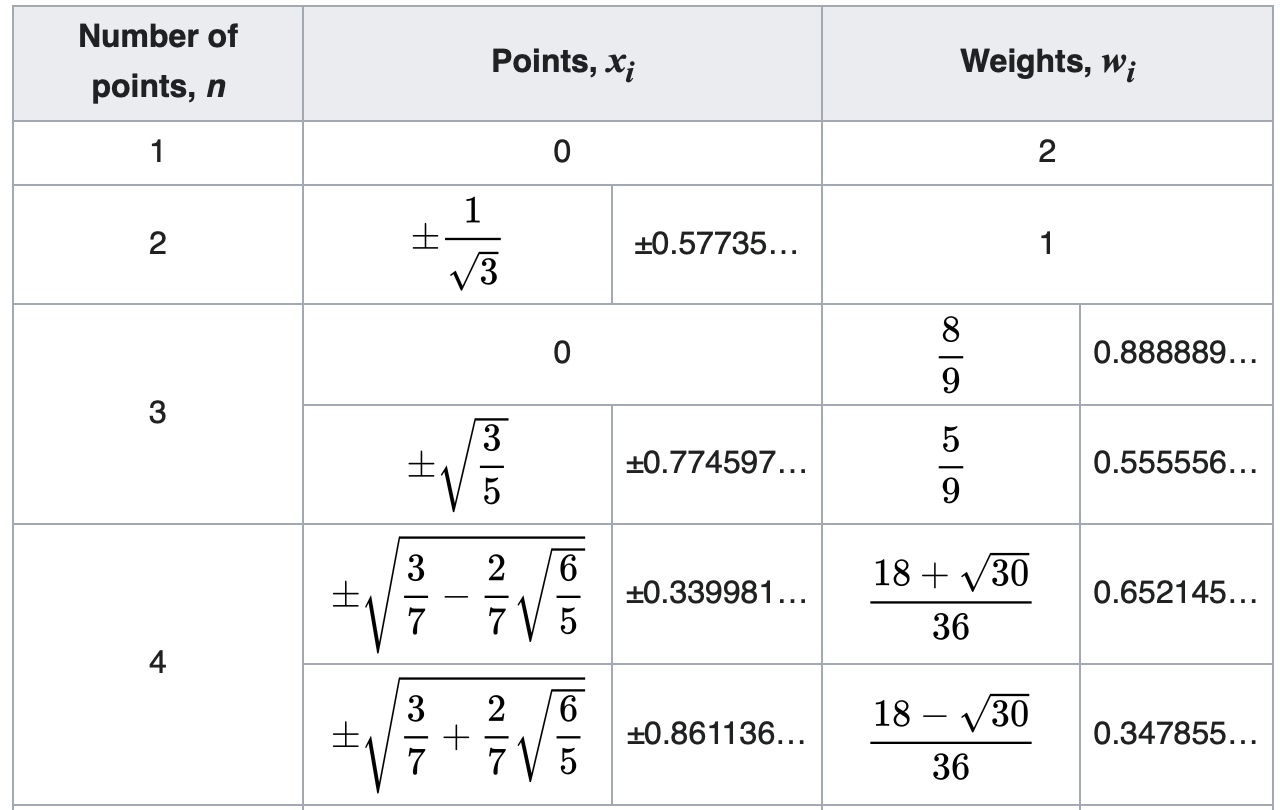
\includegraphics[width=5cm]{quadrature_table.png}

\end{center}
\end{columns}
\blfootnote{From \href{https://en.wikipedia.org/wiki/Gauss–Legendre_quadrature}{Wikipedia}}
\end{frame}
\placelogotrue

\begin{frame}{Quadrature, Part 2}
\begin{columns}
\column{0.48\linewidth}
\begin{outline}
  \1 Meshing assumes ``full'' elements 
  \1 How do we find quadrature for ``partial'' elements?
  \2 Create domain specific quadrature
  \2 OR
  \2 Manipulate weights
\end{outline}

\column{0.48\linewidth}
\begin{center}

\begin{align*}
K_{i,j} &= \int_{\Omega_e} P \phi_i' \phi_j' \ d \Omega_e \\
        &\approx \sum_{k=0}^n w_k P \phi_i'(x_k) \phi_j'(x_k)
\end{align*}

\end{center}
\end{columns}
\end{frame}


